\documentclass[12pt, a4paper, lithuanian, final]{article}

\usepackage{hyperref}
\usepackage{graphicx}
\usepackage{float}
\usepackage{placeins}
\usepackage{gensymb}
\usepackage{xcolor}
\usepackage{listings}
\usepackage{amsmath}
\usepackage{textgreek}
\usepackage{mathtools}
\usepackage[obeyFinal]{easy-todo}
\usepackage[utf8]{inputenc}
\def\LTfontencoding{L7x}
\usepackage[\LTfontencoding]{fontenc}
\usepackage[lithuanian]{babel}
%\usepackage{times}

%\renewcommand{\sfdefault}{uhv}
%\renewcommand{\rmdefault}{utm}
%\renewcommand{\ttdefault}{ucr}

\usepackage{VUMIF}

%Kodo highlitinimo configas
\lstset{basicstyle=\ttfamily,
	showstringspaces=false,
	commentstyle=\color{red},
	keywordstyle=\color{blue}
	}


% Titulinio puslapio reikalai
\vumifdept{Programų sistemų katedra}
\vumifpaper{Bakalaurinis darbas}
\title{Autonominis ketursraigčio skrydžio valdymas\\Autonomus Control of Quadcopter Flight}
\author{
    4 kurso 1 grupės studentas \\
    Rytis Karpuška
}

\supervisor{Irus Grinis, lekt.}
\reviewer{Vytautas Valaitis}
\date{Vilnius \\
	2014}


\begin{document}

%titulinis ir turinys
\maketitle
\tableofcontents



\vumifsectionnonum{Įvadas}



\section{Ketursraigčio techninė įranga}
Įprasto ketursraigčio techninė struktūra yra palyginus lengvai suprojektuojama bei pagaminama tačiau to negalima pasakyti apie programinę įrangą, bei algoritmus valdančius skrydį.



\subsection{Rėmas, varikliai ir propeleriai}
Ketursraigtis susideda iš "`X"' formos rėmo, kurio galuose yra po elektrinį bešepetėlinį variklį su propeleriu.
Priešingai nei įprastuose sraigtasparniuose, šių propelerių atakos kampas nėra reguliuojamas, o tai leidžia stipriai supaprastinti skraidyklės techninę struktūrą ir atsisakyti sudėtingų mechaninių dalių.
Varikliai skirstomi į dvi grupes iš kurių viena sukasi pagal laikrodžio rodyklę, kita -- prieš laikrodžio rodyklę.
Šių variklių sukimosi greitis yra reguliuojamas siekiant išgauti tinkamą sukamąją bei keliamąją jėgas.

\begin{figure}[H]
\begin{center}
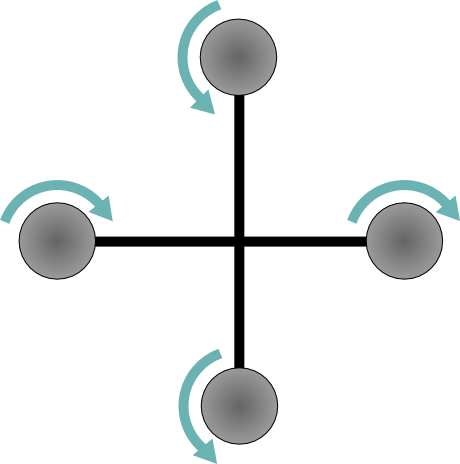
\includegraphics[width=0.5\textwidth]{img/rotor-direction.png}
\caption{Ketursraigčio rėmo ir variklių išdėstymas. Jų sukimosi kryptys.}
\end{center}
\end{figure}

Šio darbo tikslams pasiekti buvo nupirktas "`HobbyKing x525"' 600mm skersmens rėmas, pagamintas iš aliuminio ir stiklo pluošto.
Taip pat elektriniai bešepetėliniai 160W galios varikliai "`Turnigy D2822"' ir 8 colių ilgio, bei 4 laipsnių atakos kampo propeleriai.


\subsection{Valdymo elektronika}
Stabilaus skrydžio išlaikymas ketursraigtyje yra per sudėtinga užduotis žmogui (pilotui) todėl pasitelkiama pagalbinė elektronika palengvinanti ketursraigčio valdymą.

Valdymo elektronikai išskiriami tokie uždaviniai:
\begin{itemize}
	\item Skrydžio stabilizavimas bei kontrolė
	\item Ryšio su pilotu arba valdančia sistema palaikymas
	\item Sugeneruoti galios signalus reikalingus varikliams
\end{itemize}

\paragraph{Skrydžio stabilizavimas bei kontrolė}
Skrydžio stabilizavimui bei kontrolei atlikti naudojami sensoriai pagal kurių duomenis yra paskaičiuojami kokių korekcinių veiksmų reikia imtis norint įgyvendinti piloto ar valdančios sistemos komandas.
Išskiriami svarbiausi parametrai yra tikslumas bei greitis.

Atsižvelgiant į rekalavimus šiems parametrams, buvo parinktas kompanijos "`STMicroelectronics"' procesorius "`STM32F401"' bei kompanijos "`InvenSense"' sensorius "`MPU6050"'

\paragraph{Ryšio su pilotu arba valdančia sistema palaikymas}
Ryšio palaikymas parametrizuojamas pagal duomenų persiuntimo greitį ir latenciją, bei veikimo ribas.
Ketursaigčio atveju persiunčami duomenys yra tik valdymo signalai iš piloto arba valdančios sistemos, todėl buvo pasirinktas GSM ryšys.
Taip pat "`Raspberry pi"' kompiuteris su "`Linux"' operacine sistema atlikdavo viską kas reikalinga GSM ryšiui palaikyti.

\paragraph{Galios signalų generavimas}
Bešepetėliniai varikliai reikalauja trijų galio signalų jų sukimuisi palaikyti.
Šiam tiklui buvo nupirkti 18A elektroniniai greičio valdikliai galintys suvaldyti apie 200W galios, tad puikiai tinkantys 160W galios varikliams.

\begin{figure}[H]
\begin{center}
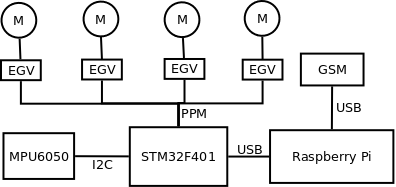
\includegraphics[width=0.5\textwidth]{img/elektronikosSchema.png}
\caption{Ketursraigčio elektronikos sudedamųjų dalių schema.}
\end{center}
\end{figure}




\section{Matematinis skrydžio modelis}



\subsection{Lokali ir globali koordinačių sistemos}
Pravartu apibrėžti lokalią ir globalią koordinačių sistemas, kuriose nagrinėsime ketursraigčio dinamiką.
Lokalioje koordinačių sistemoje x ir y ašis yra sulygiuota su ketursraigčio rėmo strypais, kur $X$ rodo pirmojo variklio kryptimi, $Y$ - antrojo.
Globali sistema yra susieta su žemės gravitaciniu laiku, ir toje sistemoje gravitacinio lauko vektorius nukreiptas priešinga $Z$ ašiai kryptimi.

\begin{figure}[H]
\begin{center}
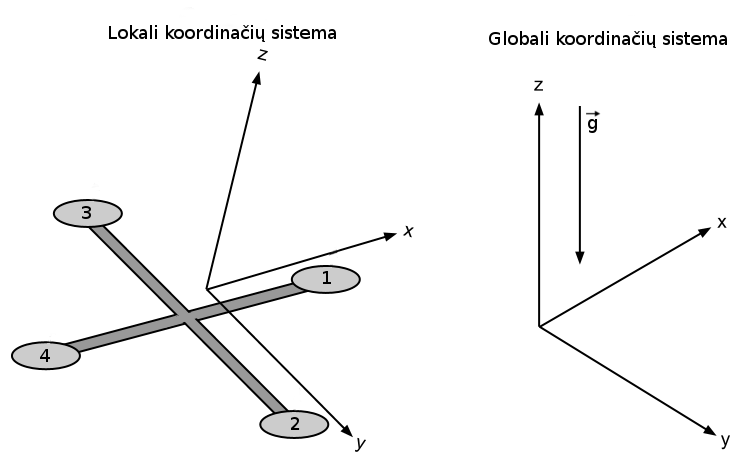
\includegraphics[width=1.0\textwidth]{img/Quadcopter_Coordinates.png}
\caption{Lokalios ir Globalios koordinačių sistemos palyginimas.}
\end{center}
\end{figure}


Konvertavimas tarp šių koordinačių sistemų bus vykdomas kvaternionų pagalba (žr.: TODO\_SKYR\_NR):

\begin{equation}
	q_{l} = q_{p} * q_{g} * q_{p}^{-1}
\end{equation}

ir į priešingą pusę:

\begin{equation}
	q_{g} = q_{p}^{-1} * q_{l} * q_{p}
\end{equation}

Čia $q_{g}$ -- tašką arba vektorių globalioje koordinačių sistemoje atvaizduojantis kvaternionas, $q_{l}$ -- tašką arba vektorių lokalioje koordinačių sistemoje atvaizduojantis kvaternionas, $q_{p}$ -- kampinės pozicijos kvaternionas (žr.: TODO\_SKYR\_NR).





\subsection{Keliamoji jėga}

Ketursaigtis sukuria keliamąją jėgą priversdamas judėti orą žemyn.
Pagal trečią niutono dėsnį, kokia jėga ketursraigtis veikia, orą, tokio pačio dydžio, tik priešingos krypties jėga oras veikia ketursraigtį.

\begin{equation}
	F_{qa} = -F_{aq}
\end{equation}

Čia $F_{qa}$ jėga, kuria ketursraigtis veikia orą, o $F_{aq}$ jėga, kuria oras veikia ketursraigtį.
Darome prielaidą, kad oras iki ketursraigčiui jį pajudinant nejudėjo, o iš to seka:

\begin{equation}
	F = m * a
\end{equation}

Čia $F = |F_{qa}|$, $m$ - oro, kuriam suteikiamas pagreidis, masė, o $a$ pagreitis suteikiamas orui.


Propelerio prastumamas oro kiekis yra tiesiogiai proporcingas propelerio sukimosi greičiui:
\begin{equation}
	A = \omega * C
\end{equation}

Čia $A$ yra oro tūris prastumtas per vieną apsisukimą, $\omega$ yra propelerio sukimosi greitis, o $C$ - konstanta priklausanti tik nuo propelerio savybių susiejanti sukimosį greitį su tūriu.

Pagal prielaidą, kad oras prieš propeleriui jį pasiekiant nejudėjo, skaičiuojame propelerio sukuriamą oro pagreitį:
\begin{equation}
	a = \dfrac{V}{\delta t}
\end{equation}

kur $V$ yra įgyjamas oro greitis prasisukus propeleriui

\begin{equation}
	a = \dfrac{ \omega * C}{\delta t}
\end{equation}

Čia C yra konstata priklausanti tik nuo nekintančių propelerio savybių.

\begin{equation}
	a = \dfrac{\omega * C}{ 1 / \omega}
\end{equation}
\begin{equation}
	a = \omega ^ 2 * C
\end{equation}










\subsection{Sukamoji jėga}





\subsection{Bendras judėjimo modelis}



\section{Kampinės padėties skaičiavimas}
\subsection{Kvaternionai}
\subsection{Kampinės padėties skaičiavimas pagal giroskopą}
\subsection{Kampinės padėties skaičiavimas pagal akselerometrą}
\subsection{Galutinis kampinės padėties radimas}



\section{Kampinės padėties valdymo algoritmas}
\subsection{PID valdymo algoritmas}
\subsection{PID pritaikymas ketursraigčio valdymui}



\section{Skrydžio valdymas}
\subsection{Atviro-ciklo valdymas}
\subsection{Kampinės pozicijos tikslų lentelė}
\subsection{Atviro-ciklo valdymo trūkumai}



\section{Programinė įranga}
\subsection{Bendroji architektūra}
\subsection{Kompiuteriui skirtas klientas}
\subsection{Retransmitorius}
\subsection{Ketursraigčio pagrindinis valdiklis}

\vumifsectionnonum{Išvados}



\bibliography{Bibliografija}
\begin{itemize}%TODO: fixme
	\item [[AAJ+01]] - \textit{Implementing a Sensor Fusion Algorithm for 3D Orientation Detection with Inertial/Magnetic Sensors}, \url{http://franciscoraulortega.com/pubs/Algo3DFusionsMems.pdf}
	\item [[SSF+11]] - \textit{A sensor fusion algorithm for an integrated angular position estimation with inertial measurement units}, \url{http://www.date-conference.com/proceedings/PAPERS/2011/DATE11/PDFFILES/IP1_06.PDF}
	\item [[MS11]] - \textit{Modeling, Design and Experimental Study for a Quadcopter System Construction}, \url{http://brage.bibsys.no/xmlui/bitstream/id/86811/uiareport.pdf}
\end{itemize}


\end{document}



